\chapter{Architecture}
\label{ch:architecture}

This chapter presents the architectural design and implementation of the \tech{ln-history} platform. 
Building upon the fundamental concepts of the \gls{ln} and its gossip protocol, 
we first define the system requirements in \autoref{sec:requirements} 
followed by an architectural overview in \autoref{sec:high-level-architecture}.
After that the structure of this chapter mirrors the data flow within the system.
We begin by analysing each component sequentially, 
from different ingestion pipelines presented in \autoref{sec:real-time-pipeline} for
real-time analysis and \autoref{sec:batch-pipeline} for bulk insertion. 
To the storage layer in \autoref{sec:database} and its two auxiliary services:
Metadata enrichment in \autoref{sec:chain-enricher} and node behaviour monitoring \autoref{sec:peer-manager}.
After that the backend \service{ln-history-api} is explained in \autoref{sec:ln-history-api}.
To work with the results, we introduce a custom client library in \autoref{sec:ln-history-python-client}
The chapter comes to an end by first discusses continuous monitoring of the system in \autoref{sec:observability}.
Ultimately, the \autoref{sec:deployment} focuses on deployment.
As architecture decisions are often based on \textit{trade-offs} some sections
conclude with a discussion about their particular design decisions. 


\section{Requirements}
\label{sec:requirements}

The status quo of (public) datasets containing gossip of the \gls{ln} is a fragmented collection
of files and repositories hosted by various researchers (see \autoref{ch:related-work}). 
These datasets lack a unified structure, varying in their serialization formats 
(e.g., raw hex-encoded dumps versus pre-parsed JSON files) and metadata quality.

The current benchmarking tool for parsing these messages is the \term{time-machine},
developed by \citeauthor{decker_lnresearch_2020}~\cite{decker_lnresearch_2020}.
The \term{time-machine} tool iterates through a file of gossip messages encoded in hex and yields a \tech{networkx} graph~\cite{hagberg_exploring_2008}.
This, simple yet, effective procedure takes around 10 minutes on commodity hardware (e.g., Apple M1, 16 GB RAM) 
to process ten million gossip messages and yields a single graph for a single timestamp.
Creating $n$ snapshots requires $n$ iterations of the \term{time-machine} tool
through every collected gossip message resulting in redundant computation.  

Further, gossip data analysis (e.g. gossip propagation lag) also needs a whole iteration through the file of gossip messages
due to the fact that no index or meta information exists for a single gossip message.

To address these limitations, the \term{ln-history} platform is designed to 
transition from linear file processing to a database-centric architecture,
indexing gossip messages and reducing the workload for various analytical queries
e.g. snapshot generation from $\mathcal{O}(n)$ to $\mathcal{O}(\log n)$ or even $\mathcal(1)$. 

The system must fulfil the following functional and non-functional requirements, 
categorized by their operational scope.

\subsection{Functional Requirements}

The requirements are divided into data storage, analysis, and real-time capability. 
Each requirement has a label which will be referenced when being taken into account in the architectural design.

\subsubsection{Data Storage \& Persistence}
\begin{enumerate}[label=\textbf{RF\arabic*}, ref=RF\arabic*, leftmargin=3.5em]
    \item \label{req:dual-format} \textbf{Dual-Format Persistence:} 
        All gossip messages must be stored in both their raw wire format (bytes) for 
        bandwidth-efficient retrieval and a parsed format (structured data) for in-depth analytical querying.
    \item \label{req:persistance} \textbf{Long-Term Persistence:} 
        The system must ensure durable storage of all collected messages, serving as a permanent archive of the \gls{ln} history.
\end{enumerate}

\subsubsection{Querying \& Historic Analysis}
\begin{enumerate}[label=\textbf{RF\arabic*}, ref=RF\arabic*, resume, leftmargin=3.5em]
    \item \label{req:snapshot} \textbf{Snapshot Retrieval:} 
        The system must return the precise set of gossip messages 
        that make up the valid network state at any given timestamp.
    \item \label{req:snapshot-diff} \textbf{Time-Window Retrieval:} 
        The system must support range queries to retrieve all messages 
        broadcast between two given timestamps $t_{start}$ and $t_{end}$.
    \item \label{req:entity-filtering} \textbf{Entity Filtering:} 
        The system must be able to filter gossip history by specific identifiers, specifically \code{node\_id} and \code{scid}.
\end{enumerate}

\subsubsection{Real-Time Operations}
\begin{enumerate}[label=\textbf{RF\arabic*}, ref=RF\arabic*, resume, leftmargin=3.5em]
    \item \label{req:ingestion} \textbf{Low-Latency Ingestion:} 
        Newly received gossip from the \gls{p2p} network must be inserted into the storage engine 
        immediately to ensure the database reflects the live state.
    \item \label{req:concurrency} \textbf{Concurrency:} 
        The system must support simultaneous operations; historic analysis queries (\gls{olap}) 
        must not block or significantly degrade the performance of real-time write operations (\gls{oltp}).
    \item \label{req:multiple-nodes} \textbf{Multiple nodes:} 
        The system must be scalable to multiple collecting nodes that feed 
        new gossip messages in parallel into the platform.
    \item \label{req:metadata}\textbf{Metadata:} 
        In addition to the gossip message itself, metadata (e.g. the collection timestamp) 
        must be linked to and stored.
    \item \label{req:batch-ingestion} \textbf{Batch Ingestion:} 
        The system must be able to insert historic messages in large batches.
\end{enumerate}


\subsection{Non-Functional Requirements}
The design is further constrained by quality attributes essential for a research tool in the Bitcoin development community.

\begin{enumerate}[label=\textbf{RN\arabic*}, ref=RN\arabic*, leftmargin=3.5em]
    \item \label{req:open-source} \textbf{Transparency \& Auditability (Open Source):} 
    Aligned with the Bitcoin ethos of \enquote{Don't trust. Verify.}, 
    the platform's source code must be fully open-source under the MIT License~\cite{opensourceinitiative_mit_1988}. 
    This ensures that the data collection methodology is transparent and 
    that results generated by the platform are scientifically reproducible by independent third parties.
    
    \item \label{req:docker} \textbf{Deployability (Containerization):} 
    To facilitate easy adoption and reproducibility, the system must be fully containerized using Docker~\cite{merkel_docker_2014}. 
    This ensures the platform is environment-agnostic, allowing it to run consistently on a developer's laptop, a university server, 
    or a cloud cluster with the potential for future orchestration via Kubernetes ~\cite{burns_borg_2016}.
    
    \item \label{req:self-host} \textbf{Efficiency (Self-Hostability):} 
    The architecture must be resource-efficient enough to run on consumer-grade hardware. 
    By lowering the barrier to entry for hosting everyone should have the opportunity to run \tech{ln-history}.

    \item \label{req:maintainability} \textbf{Maintainability:}
    The system and the underlying code must be structured to support the ongoing development. 
\end{enumerate}



\section{The Big Picture: High-Level Architecture}
\label{sec:high-level-architecture}

\citeauthor{kleppmann_designing_2017} presents the \term{Lambda Architecture} in \citetitle{kleppmann_designing_2017}
as a pattern for unifying real-time and historical data processing. 

He defines the core concept as follows:
\begin{quote}
The core idea of the lambda architecture is that incoming data should be recorded by appending immutable events to an always-growing dataset,
similarly to event sourcing. [...] The lambda architecture proposes running two different systems in parallel: 
a batch processing system [...] and a separate stream-processing system.~\cite[p.~519]{kleppmann_designing_2017}   
\end{quote}

The architecture of \tech{ln-history} implements a variation of this pattern. 
Real-time gossip messages from \gls{cln} nodes are ingested immediately while the system
simultaneously supports bulk insertion of historic gossip messages.

As the batch insertion of historic gossip messages rarely occurs, 
this process is done via a \term{backfill} script manually.
On the other hand the real-time ingestion pipeline is managed by a service called \service{gossip-processor}.

Gossip messages are stored in one central database: \service{ln-history-database}.

The \autoref{fig:architecture-high-level} illustrates the architectural design of the \tech{ln-history} platform
including both data ingestion streams: batch insertion and real-time insertion.
\begin{figure}[htbp]
    \centering
    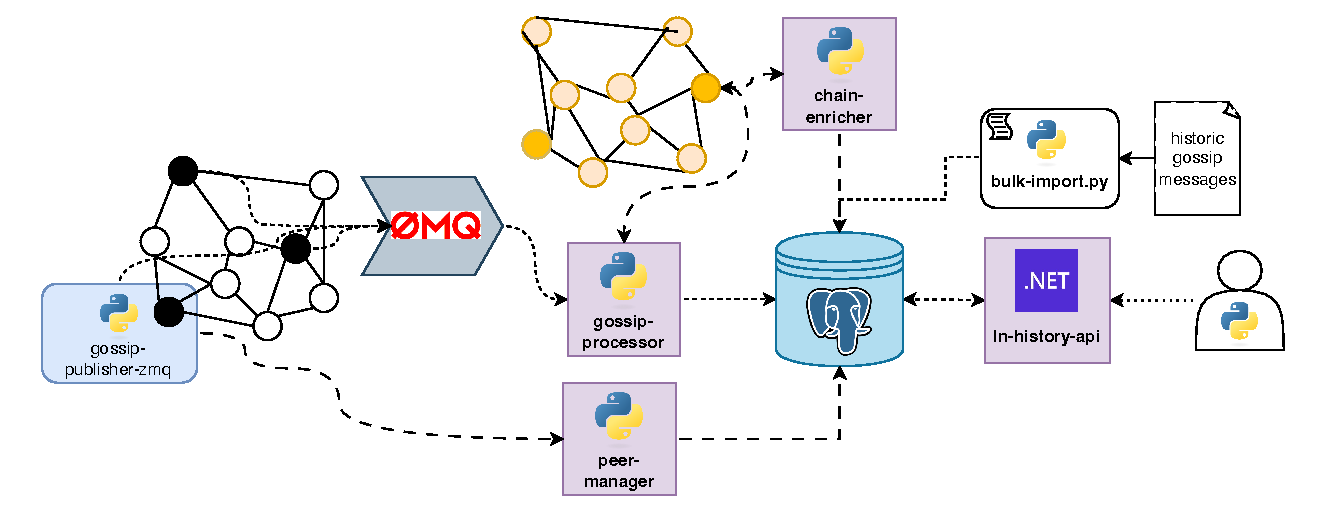
\includegraphics[width=\linewidth]{resources/images/architecture-minimal.pdf}
    \caption{High-level architecture of the \tech{ln-history} platform.}
    \label{fig:architecture-high-level}
\end{figure}

\autoref{fig:architecture-high-level} starts on the left with one or multiple 
\gls{cln} nodes indicated as filled circles which are connected to the \gls{ln} 
and run the \service{gossip-publisher-zmq} plugin.
The plugin reads the \file{gossip\_store} file and publishes new gossip messages 
enriched with additional metadata via a message queue (\tech{ZeroMQ}~\cite{hintjens_zeromq_2013}) 
to the \service{gossip\_processor} service which is indicated in purple.

The \service{gossip-processor} performs deduplication before inserting the unique 
gossip messages into the \service{ln-history-database} (coloured in blue).
Parallel to this, the \service{peer-manager} (indicated in purple) monitors every
\gls{p2p} connection for each \gls{cln} node and stores session data 
(e.g. \code{node\_id} of connected peers, session duration) into the \service{ln-history-database}.

Since the gossip messages, specifically the \code{channel\_announcement}, reference transactions 
in the Bitcoin blockchain (network is indicated in orange), 
metadata like the \code{funding\_timestamp} and \code{capacity\_sat} get retrieved externally. 
This is handled by the \service{chain-enricher} service (coloured in purple), 
which monitors the \service{ln-history-database} for those missing values.
The service extracts the \code{timestamp}\footnote{
    A block's \code{timestamp} does not necessarily represent its exact discovery time. 
    Under Bitcoin consensus rules, a timestamp is valid as long as it is strictly greater than the median 
    of the previous 11 blocks and no more than two hours ahead of the network time~\cite{bitcoincoredevelopers_bitcoin_2026a}.
} 
from the block that mined the funding transaction. It then waits for the channel
to reach the required maturity before fully enriching the database\footnote{
    A Lightning channel is not instantly valid for public routing as soon as the funding block is found. 
    According to the BOLT 7 specification, nodes must wait until the funding transaction achieves 
    at least six confirmations before broadcasting a \code{channel\_announcement}~\cite{lightningdevelopers_bolts_2018}.
}.

Lastely the \service{ln-history-api} queries the \tech{ln-history-database} 
and provides a \term{restful} API for in-depth analysis as well as secure authentication\footnote{
The \textit{SwaggerUI} shows the endpoints \url{https://api.ln-history.info/swagger/index.html}}.

On the right-hand side clients (users) request the \service{ln-history-api}. 
The \service{ln-history-python-client} provides the functionality to easily parse the response into readable formats.
To minimize bandwidth, large results like a snapshot, are sent in raw bytes following the format of \gls{ln} gossip messages.
The \service{ln-history-python-client} parses the raw bytes and returns a graph object useful for further analysis.
Additional functions to work with the \service{ln-history-api} are provided.



\section{Real-Time Ingestion Pipeline}
\label{sec:real-time-pipeline}

As described by \citeauthor{hohpe_enterprise_2012} in \citetitle{hohpe_enterprise_2012} 
the \term{Pipes and Filters} architectural style should be used to
\enquote{divide a larger processing task into a sequence of smaller independent processing steps (filters)
 that are connected by channels (pipes)}~\cite[p.~70]{hohpe_enterprise_2012}.

Adopting this pattern, the \service{gossip-publisher-zmq} plugin acts as the initial filter, 
validating the authenticity of incoming gossip messages at the \gls{cln} node level. 
Validated messages are then transmitted via a \tech{ZeroMQ} message queue to the \service{gossip-processor} service. 
The downstream component performs deduplication before persisting into the \service{ln-history-database}.

\subsection{\service{Gossip-Publisher-Zmq}}
The \service{gossip-publisher-zmq} plugin serves as the starting point for the pipeline. 
It is written in \tech{Python}~\cite{pythonsoftwarefoundation_python_2025} and 
the source code is available at~\cite{kraus_gossippublisherzmq_2026},
aligning with the requirement for open-source transparency (\ref{req:open-source}).
The plugin interfaces directly with the \gls{cln} architecture, following the 
official plugin documentation~\cite{corelightningdevelopers_cln_2026}.

\subsubsection{Data Source: The Gossip Store}
The \gls{cln} architecture delegates gossip management to the \term{gossipd deamon}. 
This process persists all gossip into a specialized append-only log file known as the \file{gossip\_store}. 
Every collected message is stored as a \term{record}, encapsulating the raw gossip payload within a structural wrapper.

The file begins with a \qty{1}{\byte} \term{File Header}. 
The top \qty{3}{\bit} encode the major version (currently \num{0}), 
while the lower \qty{5}{\bit} encode the minor version (currently \num{15}). 
Following this header, the file consists of a sequence of records. 

\begin{figure}[htbp]
    \centering
    \begin{bytefield}[bitwidth=0.8em, endianness=big]{32}
        \bitheader{0, 15, 16, 31} \\
        
        \begin{rightwordgroup}{Record Header\\(\qty{12}{\byte})}
            \bitbox{16}{\code{flags} (be16)} &
            \bitbox{16}{\code{len} ($L$) (be16)} \\
            \bitbox{32}{\code{crc} (be32)} \\
            \bitbox{32}{\code{timestamp} (be32)}
        \end{rightwordgroup} \\
        
        \begin{rightwordgroup}{Message Body\\($L$ bytes)}
            \bitbox{16}{\code{type} (be16)} &
            \bitbox[lrt]{16}{Start of Gossip Data \dots} \\
            \skippedwords \\
            \bitbox[lrb]{32}{...End of Data ($L-2$ bytes)}
        \end{rightwordgroup}
    \end{bytefield}
    \caption{Byte layout of a single record within the \gls{cln} \file{gossip\_store} file. 
            The record consists of a \qty{12}{\byte} internal header followed by the variable-length Lightning message payload. 
            All multibyte integers are stored in \gls{be} format~\cite{corelightningdevelopers_cln_2026}.}
    \label{fig:core-lightning-gossip-store-bytefield}
\end{figure}

The byte layout of an individual record is depicted in \autoref{fig:core-lightning-gossip-store-bytefield}.

\subsubsection{Retrieval Logic}
To monitor the network in real-time, the plugin opens a read-only binary handle to the 
\file{gossip\_store} file and maintains a pointer to the current file offset.

When new data is appended by the \term{gossipd daemon}, the plugin advances the file handle to read the \code{record.header}. 
It extracts the payload length ($L$) from the \code{len} field (a fixed \code{be16} integer). 
It then reads the subsequent $L$ bytes to retrieve the full message body.
Before processing, the system computes the \gls{crc32} checksum of the payload and 
compares it against the \code{record.header.crc} field to ensure data integrity.

\subsubsection{Serialization and Transmission}
After successful validation, the raw message is parsed and wrapped into a structured dictionary.

\begin{listing}[htbp]
    \begin{minted}[frame=lines, fontsize=\footnotesize]{python}
    class PluginEventMetadata(TypedDict):
        type: int
        name: str
        timestamp: int
        sender_node_id: str
        length: int  # Length in bytes without starting 2-byte type

    # Base structure for all events
    class BasePluginEvent(TypedDict):
        metadata: PluginEventMetadata
        raw_hex: str
    \end{minted}
    \caption{
        Python \code{TypedDict} definitions used as a wrapper for gossip events 
        by the \service{ln-history-python-client}~\cite{kraus_lnhistorypythonclient_2026}.
    }
    \label{lst:python-dto}
\end{listing}

\autoref{lst:python-dto} shows the \gls{dto} used in the \tech{ln-history} platform.
Metadata like the \code{sender\_node\_id} which can be set via environment variables (defaults to its own \code{node\_id}),
the \code{timestamp} when the \term{gossipd deamon} collected the message
and the length (not accounting for the \qty{2}{B} type header) of the raw message
get added to the beginning of the payload.

Finally, the structured event is broadcasted via the \tech{ZeroMQ} message queue. 
On Startup the plugin initializes a \term{PUB socket} using the host and port defined in the environment variables 
making asynchronous consumption by downstream consumers (e.g. \service{gossip-processor}) possible.


\subsection{\service{Gossip Processor}}
The \service{gossip-processor} is written in \tech{Python} and the source code can be found at ~\cite{kraus_gossipprocessor_2026}. 
It acts as a \term{SUB node}, connecting to one or more \tech{ZeroMQ} \term{PUB sockets} to consume the plugin events.
The plugin events get analysed and added into the \service{ln-history-database}.


\subsubsection{Real-time ingestion}
By utilizing a concurrent architecture, the \service{gossip-processor} can consume gossip messages 
from the network without blocking database write operations, ensuring low-latency ingestion (\ref{req:ingestion}).

The database worker continuously dequeues messages, aggregating them into batches of a configurable size 
(governed by the \code{BATCH\_SIZE} environment variable, which defaults to $200$).
Each batch is encapsulated within a single atomic transaction, ensuring data integrity in the event of a failure.

Message processing begins by storing the observation metadata (\ref{req:metadata}). 
The \code{gossip\_id}, \code{collector\_node\_id}, and the \code{seen\_at} 
timestamp are inserted into the \code{gossip\_observations} table 
tracking exactly when and by which collector node the message was seen, 
seamlessly allowing the system to scale to multiple collecting nodes (\ref{req:multiple-nodes}).

As a next step the gossip message gets upserted (create a new row or update if it exists) into the \code{gossip\_inventory} table.
If the \code{gossip\_id} is already present in the table, the query yields a \code{rowcount} of $0$, 
meaning that the gossip message is a duplicate and does not need to be further processed.

The processing branches depending on the specific gossip message type:

\paragraph{Channel Announcements}
For each \code{channel\_announcement} the \service{gossip-processor} checks foreign key constraints 
by ensuring both participating \code{node\_id}s exist in the \code{nodes} table, inserting them if they are missing.
After that, the channel is inserted into the \code{channels} table. 
While the raw message data is persisted alongside the parsed attributes, fulfilling the dual-format requirement (\ref{req:dual-format}), 
attributes derived from the underlying Bitcoin funding transaction (\code{capacity\_sat} and \code{funding\_timestamp})
are not part of BOLT\#7 messages (as discussed in \autoref{sec:gossip-messages}),
these fields are temporarily left null and are populated asynchronously by the \service{chain-enricher}.

\paragraph{Node Announcement}
Every \code{node\_announcement} messages, contains information about the sending node.
This node is upserted into the \code{nodes} table, 
updating the \code{last\_seen} timestamp upon conflict.
Since only one \code{node\_announcement} message is valid at a given timestamp, 
each message gets \code{valid\_from} and \code{valid\_to} boundaries.
When a new announcement supersedes an older one, 
the previous record's \code{valid\_to} timestamp is closed.
Due to the asynchronous nature of \gls{p2p} networks, messages can arrive out of order. 
If the \code{node\_announcement} message has a \code{timestamp} older than that of the latest,
the \service{gossip-processor} identifies it as historical data and queries the \service{ln-history-database}
to find the appropriate gap and limit the message's \code{valid\_to} boundary.

\paragraph{Channel Update}
Because \code{channel\_updates} also require temporal boundaries, 
they are processed using the same logic as \code{node\_announcements}. 
Additionally, the \service{gossip-processor} must be capable of handling \term{orphan} updates. 
These are \code{channel\_update} messages that reference a channel not (yet) registered in the \code{channels} table. 
Since a \code{channel\_update} does not contain the public keys of the participating nodes, 
it is impossible to deduce the network topology and automatically create a placeholder channel. 
Therefore, once fundamental constraints (such as the \code{gossip\_id}) are satisfied, 
the message is persisted in the \code{channel\_updates} table, but the relational 
link to a specific channel via the \code{scid} remains unestablished.

\subsubsection{Discussing Throughput Performance}

As stated in \citetitle{kleppmann_designing_2017} thinking about performance and scaling should not be the first objective.
He advocates to focus on getting things working first.~\cite[Chapter~1]{kleppmann_designing_2017}

Following this principle the initial design processed one gossip message at a time.
This approach simplified the insertion logic massively, 
but it generated an unsustainable volume of read and write operations against the \service{ln-history-database}.
Depending on the specific message type, processing a single gossip message required between three and six individual database queries.
During peak network activity, where the volume reaches an order of magnitude of $100$ gossip messages per second, 
this sequential approach exhausted the database's capacity due to high random disk I/O.

The operation of only two collector nodes already induced a cumulative processing lag 
and made the database throughput the primary bottleneck for scalability \tech{ln-history}.

To resolve this limitation, the ingestion pipeline was refactored to aggregate gossip messages into batches,
that are executed within a single atomic database transaction.

This architectural upgrade reduced the transaction overhead and the frequency of disk writes, 
yielding improvements in the overall throughput and enabling scaling.


\section{The Batch Ingestion Pipeline}
\label{sec:batch-pipeline}
The batch ingestion pipeline is done via a \tech{Python} script called \file{bulk-import.py} 
and the source code found at\footnote{\url{https://ln-history.info/bulk-import.py}}.

Because historic imports are rare, high-volume operations applied to bounded datasets, 
a dedicated batch processing script is utilized to fulfil the batch ingestion requirement (\ref{req:batch-ingestion}).
As outlined by \citeauthor{kleppmann_designing_2017}~\cite{kleppmann_designing_2017}, 
batch processing frameworks maximize throughput by avoiding random, individual database writes. 

Unlike the real-time \service{gossip-processor}, which relies on the database for conflict resolution, 
this script optimizes performance by performing data grouping and temporal boundary calculations 
entirely in memory prior to executing bulk database inserts. It achieves this using a two-pass algorithm.


\paragraph{Step 1: Parsing and Aggregation}
In the first pass, the script sequentially processes the provided file of binary-encoded 
gossip messages (denoted as \term{historic gossip messages} in \autoref{fig:architecture-high-level}).
The messages are extracted and parsed utilizing the \code{ln-history-python-client}, 
which is detailed further in \autoref{sec:ln-history-python-client}.

he script tracks the \code{first\_seen} and \code{last\_seen} timestamps during the extraction
for every encountered \code{node\_id} and temporarily caches \code{channel\_announcement} messages in memory.

Because historical dumps inherently lack metadata regarding which specific collector node received the message, 
the script utilizes a configured environment variable (\code{HISTORIC\_COLLECTOR\_NODE\_ID} 
\footnote{defaults to \code{01000000000000000000000000000000}}) to inject dummy collector node values. 
This allows the script to successfully reconstruct the required relations and insert every parsed message
into both the \code{gossip\_inventory} and \code{gossip\_observations} tables.


\paragraph{Step 2: Temporal Boundary Computation}
To construct the historical timeline, the script groups all \code{channel\_updates} and \code{node\_announcements}
by their respective identifiers (\code{scid} and \code{node\_id}) and sorts them chronologically. 
By iterating through these sorted lists, the script computes the \code{valid\_to} boundary for each message 
based on the \code{valid\_from} timestamp of the subsequent message. 
During this pass, it also compares adjacent records to flag whether a \code{channel\_update} is
a fee change (\code{is\_fee\_update}) or a routing change (\code{is\_topology\_update}).
Once the temporal state is completely constructed in memory, 
the script flushes the formatted data into the PostgreSQL database using high-performance batch operations.

Ultimately, an asynchronous backfill query aligns the \code{internal\_id} fields across the content tables.

\paragraph{Discussing Limitations of Bulk insertion}
The whole \term{historic gossip messages} file is loaded in memory which is its primary limitation. 
During the initial parsing phase, the entire \term{historic gossip messages} dataset is loaded and aggregated in memory.
The executing machine must possess sufficient Random Access Memory (RAM) to accommodate these massive data structures.

Depending on the machine that executes the \file{bulk-import.py} script, enough memory must be provided.
Attempting to process a multi-gigabyte file can result in \gls{oom} exceptions, which causes the batch insertion pipeline to crash.
Partitioning the file into sequential chunks of one single gigabyte prior to insertion, will mitigate this.


\section{Database: \service{ln-history-database}}
\label{sec:database}

This section focuses on the persistence responsible for storing the collected gossip data. 
We detail the data model, including major indices as well as the physical layout,
and finish with a discussion about the configuration of the \service{ln-history-database}. 


\subsection{Data Model}
The data model of the \service{ln-history-database} is grouped into four logical domains: 
\textit{Master Registry and Observations}, \textit{Content Tables}, 
\textit{Closure Analysis}, and \textit{Peer Operations}. 

\subsubsection{Master Registry and Observations}
% Master Registry & Observations
\begin{figure}[H]
    \centering
    \begin{tikzpicture}[node distance=1.5cm and 2.5cm]

        % 1. Gossip Inventory (The Anchor)
        \node[dbtable] (inventory) {
            \begin{tabular}{l l}
                \rowcolor{blue!15} \multicolumn{2}{c}{\textbf{gossip\_inventory}} \\
                \textbf{PK} & \code{gossip\_id} \\
                \textbf{FK} & \code{internal\_id} \\
                & \code{type} \\
                & \code{first\_seen\_at} \\
            \end{tabular}
        };

        % 2. Gossip Observations
        \node[dbtable, below=of inventory] (observations) {
            \begin{tabular}{l l}
                \rowcolor{gray!15} \multicolumn{2}{c}{\textbf{gossip\_observations}} \\
                \textbf{PK} & \code{gossip\_id} \\
                \textbf{FK} & \code{internal\_id} \\
                \textbf{FK} & \code{collector\_node\_id} \\
                & \code{seen\_at} \\
                & \code{sender\_timestamp} \\
            \end{tabular}
        };

        % 3. Collectors
        \node[dbtable, right=of observations] (collectors) {
            \begin{tabular}{l l}
                \rowcolor{gray!15} \multicolumn{2}{c}{\textbf{collectors}} \\
                \textbf{PK} & \code{node\_id} \\
                & \code{alias} \\
                & \code{total\_messages...} \\
            \end{tabular}
        };

        % Relationships
        \draw[relation] (observations.north) -- (inventory.south) 
            node[midway, left, font=\scriptsize] {1:N};
        \draw[relation] (observations.east) -- (collectors.west)
            node[midway, above, font=\scriptsize] {1:N};

    \end{tikzpicture}
    \caption{
        \textit{Master Registry and Observations}: The \code{gossip\_inventory} 
        acts as the immutable ledger, while \code{gossip\_observations} links 
        messages to the specific \code{collectors} that received them.
    }
    \label{fig:db-master-registry}
\end{figure}
~
The centre of the data model is shown in\autoref{fig:db-master-registry} and begins with 
the \code{gossip\_inventory} table, which functions as an append-only ledger. 
It registers every unique message via its \code{gossip\_id} and assigns a strictly monotonically increasing \code{internal\_id}. 

The \code{gossip\_id} is the \code{SHA256} hash of the raw bytes of the gossip message. 
Due to the nature of this hashing function, a collision is statistically almost impossible to occur,
making this a viable option to uniquely identify and reference a gossip message.

As advocated by \citeauthor{kleppmann_designing_2017}~\cite[Chapter~3]{kleppmann_designing_2017}, 
structuring the core database as an append-only log of immutable events ensures 
robust data integrity and prevents the loss of historical context, 
fulfilling the need for long-term persistence (\ref{req:persistance}).


\subsubsection{Content Tables}
% Content Tables (SCD Type 2)
\begin{figure}[H]
    \centering
    \begin{tikzpicture}[node distance=1.2cm and 0.5cm]

        % 1. Nodes (Top Center)
        \node[dbtable] (nodes) {
            \begin{tabular}{l l}
                \rowcolor{orange!15} \multicolumn{2}{c}{\textbf{nodes}} \\
                \textbf{PK} & \code{node\_id} \\
                & \code{first\_seen} \\
                & \code{last\_seen} \\
            \end{tabular}
        };

        % 2. Node Announcements (Below Left of Nodes)
        \node[dbtable, below left=1cm and 0.5cm of nodes] (nodeann) {
            \begin{tabular}{l l}
                \rowcolor{green!15} \multicolumn{2}{c}{\textbf{node\_announcements}} \\
                \textbf{PK, FK} & \code{gossip\_id} \\
                \textbf{FK} & \code{node\_id} \\
                & \code{valid\_from} \\
                & \code{valid\_to} \\
                & \code{is\_data\_update} \\
                & \code{raw\_gossip} \\
            \end{tabular}
        };

        % 3. Channels (Below Right of Nodes)
        \node[dbtable, below right=1cm and 0.5cm of nodes] (channels) {
            \begin{tabular}{l l}
                \rowcolor{orange!15} \multicolumn{2}{c}{\textbf{channels}} \\
                \textbf{PK, FK} & \code{gossip\_id} \\
                \textit{U} & \code{scid} \\
                \textbf{FK} & \code{source\_node\_id} \\
                \textbf{FK} & \code{target\_node\_id} \\
                & \code{capacity\_sat} \\
            \end{tabular}
        };

        % 4. Gossip Inventory Anchor (Bottom Left, directly below node_announcements)
        \node[dbtable, dashed, below=1cm of nodeann] (inventory2) {
            \begin{tabular}{l l}
                \rowcolor{blue!10} \multicolumn{2}{c}{\textit{gossip\_inventory}} \\
                \textbf{PK} & \code{gossip\_id} \\
            \end{tabular}
        };

        % 5. Channel Updates (Bottom Right, directly below channels)
        \node[dbtable, below=1cm of channels] (chanupd) {
            \begin{tabular}{l l}
                \rowcolor{green!15} \multicolumn{2}{c}{\textbf{channel\_updates}} \\
                \textbf{PK, FK} & \code{gossip\_id} \\
                \textbf{FK} & \code{scid} \\
                & \code{direction} \\
                & \code{valid\_from} \\
                & \code{valid\_to} \\
                & \code{is\_fee\_update} \\
            \end{tabular}
        };

        % Relationships 
        
        % Solid links (Entity relations)
        \draw[relation] (nodeann.north) -- (nodes.south west);
        \draw[relation] (channels.north) -- (nodes.south east) 
            node[midway, right, font=\scriptsize, xshift=2pt] {source / target};
        \draw[relation] (chanupd.north) -- (channels.south);
        
        % Dashed links (Back to Anchor)
        \draw[relation, dashed] (nodeann.south) -- (inventory2.north);
        \draw[relation, dashed] (chanupd.west) -- (inventory2.east);
        \draw[relation, dashed] (channels.south west) -- (inventory2.north east);

    \end{tikzpicture}
    \caption{
        \textit{Content Tables}: This domain implements the \gls{scd} Type 2 architecture. 
        While the temporal boundaries for gossip messages are defined as \code{valid\_from} and \code{valid\_to} 
        in the \code{node\_announcements} and \code{channel\_updates} tables, the \code{channels} table 
        utilizes \code{funding\_timestamp} and \code{closing\_timestamp}.
        All content tables enforce a foreign key relationship back to the \code{gossip\_inventory}.
    }
    \label{fig:db-content-tables}
\end{figure}

The fundamental topological state of the \gls{ln} is preserved within the following tables: 
\code{nodes}, \code{channels}, \code{node\_announcements}, and \code{channel\_updates}
as shown in \autoref{fig:db-content-tables}.

Because the \tech{ln-history} platform is designed to reconstruct historical snapshots,
these tables implement a \gls{scd} Type 2 architecture that allows retaining multiple 
versioned records allows any past state to be accurately derived~\cite[Chapter~11]{kleppmann_designing_2017}. 

Mutable records such as \code{node\_announcements} and \code{channel\_updates} 
are versioned by two boundaries: \code{valid\_from} and \code{valid\_to} 
(\code{channel\_announcements} with \code{funding\_timestamp} and \code{closing\_timestamp}).
These timestamp boundaries ensure that the full topological history is immutably preserved.


\subsubsection{Closure Analysis}
% Closure Analysis
\begin{figure}[H]
    \centering
    \begin{tikzpicture}[node distance=1.5cm and 2cm]

        % 1. Channel Closures
        \node[dbtable] (closures) {
            \begin{tabular}{l l}
                \rowcolor{red!15} \multicolumn{2}{c}{\textbf{channel\_closures}} \\
                \textbf{PK, FK} & \code{gossip\_id} \\
                & \code{closing\_txid} \\
                & \code{closing\_height} \\
                & \code{closing\_timestamp} \\
                & \code{type} \\
                & \code{settled\_balance\_sat} \\
                & \code{mining\_fee\_sat} \\
            \end{tabular}
        };

        % 2. Channels Anchor (Visual link to Content Tables)
        \node[dbtable, dashed, left=of closures] (channels_anchor) {
            \begin{tabular}{l l}
                \rowcolor{orange!10} \multicolumn{2}{c}{\textit{channels}} \\
                \textbf{PK} & \code{gossip\_id} \\
            \end{tabular}
        };

        % Relationships
        \draw[relation, dashed] (closures.west) -- (channels_anchor.east) 
            node[midway, above, font=\scriptsize] {1:1};

    \end{tikzpicture}
    \caption{
        \textit{Closure Analysis}: The \code{channel\_closures} table stores on-chain settlement data. 
        It is directly linked to the \code{channels} table via the \code{gossip\_id} of the original funding announcement.
    }
    \label{fig:db-closure-analysis}
\end{figure}
The closing transaction reveals information about the channel, that is retrieved
from the Bitcoin blockchain and stored in the \code{channel\_closure} table
which links in a \textit{1:1} relationship to the \code{channels} table
as can be seen in the \autoref{fig:db-closure-analysis}.  


\subsubsection{Peer Operations}
% Peer Operations
\begin{figure}[H]
    \centering
    \begin{tikzpicture}[node distance=1.2cm and 1.5cm]

        % 1. Observed Peers (Top)
        \node[dbtable] (observed) {
            \begin{tabular}{l l}
                \rowcolor{cyan!15} \multicolumn{2}{c}{\textbf{observed\_peers}} \\
                \textbf{PK} & \code{node\_id} \\
                & \code{first\_connected\_at} \\
                & \code{last\_connected\_at} \\
            \end{tabular}
        };

        % 2. Peer Sessions (Middle)
        \node[dbtable, below=of observed] (sessions) {
            \begin{tabular}{l l}
                \rowcolor{cyan!15} \multicolumn{2}{c}{\textbf{peer\_sessions}} \\
                \textbf{PK} & \code{id} \\
                \textbf{FK} & \code{collector\_node\_id} \\
                \textbf{FK} & \code{peer\_node\_id} \\
                & \code{connected\_at} \\
                & \code{disconnected\_at} \\
            \end{tabular}
        };

        % 3. Peer Addresses (Bottom)
        \node[dbtable, below=of sessions] (paddresses) {
            \begin{tabular}{l l}
                \rowcolor{cyan!15} \multicolumn{2}{c}{\textbf{peer\_addresses}} \\
                \textbf{PK} & \code{id} \\
                \textbf{FK} & \code{session\_id} \\
                \textbf{FK} & \code{type\_id} \\
                & \code{address} \\
                & \code{port} \\
            \end{tabular}
        };

        % 4. Collectors Anchor (Left of Sessions)
        \node[dbtable, dashed, left=of sessions] (collectors_anchor) {
            \begin{tabular}{l l}
                \rowcolor{gray!10} \multicolumn{2}{c}{\textit{collectors}} \\
                \textbf{PK} & \code{node\_id} \\
            \end{tabular}
        };
        
        % 5. Address Types Anchor (Right of Addresses)
        \node[dbtable, dashed, right=of paddresses] (addrtypes_anchor) {
            \begin{tabular}{l l}
                \rowcolor{gray!10} \multicolumn{2}{c}{\textit{address\_types}} \\
                \textbf{PK} & \code{id} \\
            \end{tabular}
        };

        % Relationships 
        
        % Solid links (Entity relations)
        \draw[relation] (sessions.north) -- (observed.south) 
            node[midway, right, font=\scriptsize] {peer};
        \draw[relation] (paddresses.north) -- (sessions.south);
        
        % Dashed links (Back to Anchors)
        \draw[relation, dashed] (sessions.west) -- (collectors_anchor.east) 
            node[midway, above, font=\scriptsize] {collector};
        \draw[relation, dashed] (paddresses.east) -- (addrtypes_anchor.west);

    \end{tikzpicture}
    \caption{
        \textit{Peer Operations}: This domain tracks real-time connectivity. 
        A \code{peer\_session} records the exact timeframe a connection was 
        active between an \code{observed\_peer} and an internal \code{collector}.
    }
    \label{fig:db-peer-ops}
\end{figure}

The \gls{cln} nodes regularly switch between peers to receive gossip messages.
To persist this information, specifically the session data, the data model shown in
\autoref{fig:db-peer-ops} is deployed in the \service{ln-history-database}.



\subsection{Indexing}
To satisfy the dual requirements of high-throughput real-time ingestion (\gls{oltp}) 
and complex historical analysis (\gls{olap}) without blocking each other (\ref{req:concurrency}), 
the schema employs custom B-Tree indexes.

B-Trees are the industry standard for database indexing, providing logarithmic time complexity 
for both exact matches and range queries~\cite[Chapter~14]{garcia-molina_database_2009}.
Primary keys enforce referential integrity across the database, ensuring that duplicate \code{gossip\_id}s are always rejected.

Beyond structural constraints, composite indexes are heavily utilized to accelerate snapshot queries. 
For example, the \code{channel\_updates} table owns the \code{idx\_chan\_upd\_lookup} index on the column triple \code{(scid, direction, valid\_to)}, 
as well as the \code{idx\_chan\_upd\_validity} index combining \code{(valid\_from, valid\_to)}. 
Likewise, the \code{node\_announcements} table utilizes the \code{idx\_node\_ann\_validity} index on \code{(valid\_from, valid\_to)}
and the \code{channel\_announcements} table \code{idx\_chan\_val\-id\-ity} on \code{(funding\_timestamp, closing\_timestamp)}.

Joining tables is a necessary operation for in-depth analytical queries 
but can rapidly become a performance bottleneck if executed on suboptimal data types~\cite[Chapter~15]{garcia-molina_database_2009}.
Using the \code{gossip\_id}, which is a \code{SHA256} hash, is of datatype \code{varchar(64)}, 
as a joining column is significantly more expensive than joining on a \code{bigint} column. 
The reason for this is, that string comparisons require sequential byte-by-byte evaluation. 
Therefore, an \code{internal\_id} of type \code{bigint} (\tech{PostgreSQL}'s native 8-byte integer) 
was introduced as the primary joining key. 
Integer comparisons are executed natively at the CPU register level, 
yielding orders of magnitude faster join operations~\cite[Chapter~15]{garcia-molina_database_2009}.


\subsection{Clustering}
The data retrieval for historical snapshots is exceptionally fast due to the utilization 
of the \tech{PostgreSQL} \code{CLUSTER} command~\cite{cluster_postgresql_2026}.
While standard B-Tree indexes optimize the logical search path, they do not dictate the physical storage layout on the hard drive. 
Over time, as out-of-order gossip messages are ingested and historical gaps are filled, the tables naturally suffer from physical fragmentation.

By executing the \code{CLUSTER} command against the temporal validity indexes (such as \code{idx\_chan\_upd\_validity}), 
the database physically reorders the table rows on disk to perfectly mirror the logical index sequence. 
As detailed by Garcia-Molina et al.~\cite[Chapter~13]{garcia-molina_database_2009}, 
this physical clustering ensures that the physical location of a row correlates with the logical value of the \code{valid\_from} column.
The correlation is a value in the interval $[-1,1]$. 
As long as it is close to $-1$ or $1$ the physical value is close to 
Consequently, when analytical queries request vast time-windows of the network's history, 
the database can fetch the requested data utilizing highly efficient, sequential disk I/O reads, 
skipping random disk seeks.



\section{Data Enrichment}

\subsection{Data Enrichment from the Blockchain \service{chain-enricher}}
\label{sec:chain-enricher}

The operational footprint of the \gls{ln} on the Bitcoin blockchain is limited to two events: 
the \textit{funding} and the \textit{closing} of a channel. 

Because Lightning nodes rely on their underlying Bitcoin nodes to observe these events, 
specific on-chain metrics such as channel capacity or closure details
are omitted from the gossip protocol to reduce network bandwidth~\cite{antonopoulos_mastering_2021}.

The motivation for the \service{chain-enricher} is to seperate the gathering of on-chain information from the \service{gossip-processor}. 
The \service{chain-enricher} is written in python and its source code can be found here~\cite{kraus_chainenricher_2026}. 
It operates via concurrent worker threads that asynchronously query indexed blockchain data, 
enriching the \service{ln-history-database} with metadata without disturbing the real-time gossip ingestion.

\subsubsection{Funding Transaction Resolution}
To retrieve missing funding data, the \service{chain-enricher} continuously polls 
the database for channels lacking capacity or funding timestamp information. 
To optimize retrieval latency, the enrichment process is divided into a high-performance primary workflow (\term{fast path}) 
and a secondary fallback mechanism (\term{slow path}), 
determined by the availability of the participating nodes' on-chain public keys.

\paragraph{Primary Retrieval (Fulcrum Indexer)}
If both \code{bitcoin\_key\_1} and \code{bitcoin\_key\_2} are present in the channel's gossip data, 
the funding worker utilizes the fast path. 
It reconstructs the channel's 2-of-2 multisignature \gls{p2wsh} address by sorting the raw keys lexicographically 
in accordance with BIP67 rules~\cite{kerin_bip_2015}, and hashing the resulting witness script. 
Using this derived script hash, the enricher queries \tech{Fulcrum}~\cite{culianu_cculianu_2026}, 
a high-speed Electrum server implementation that maintains a fast, queryable index of the entire Bitcoin blockchain. 
By evaluating the transaction history of this script hash, the earliest confirmed entry is identified as the funding transaction. 
To maximize throughput, these queries are executed concurrently across multiple threads.

\paragraph{Fallback Retrieval (Bitcoin Core RPC)}
If the primary retrieval fails, the service falls back to a secondary method that leverages the structural properties of the \gls{scid}. 
As elaborated in \autoref{sec:gossip-messages}, the $64$-bit \gls{scid} deterministically encodes the block height, transaction index, and output index. 
The worker decodes this identifier and issues a sequence of batched JSON-RPC queries (\code{getblockhash}, \code{getblock}, and \code{getrawtransaction}) 
directly to a local Bitcoin Core node to locate the exact funding output.

Independently of the retrieval path utilized, the raw transaction is parsed to extract the value of the 
specific output (\code{capacity\_sat}) and the block confirmation time (\code{funding\_timestamp}). 
These metrics are then persisted into the \code{channels} table.

\subsubsection{Closure Detection and Classification}
Detecting when and how a channel is closed via raw blockchain data is highly resource-intensive, 
as it would natively require exhaustive \gls{utxo} set lookups. 
A more scalable closure detection is utilized by the \service{chain-enricher} by again using the \tech{Fulcrum} index.

For every active channel in the database with known Bitcoin keys, the closure worker utilizes the previously discussed \gls{p2wsh} script hash derivation. 
By querying \tech{Fulcrum} for the transaction history of this specific script hash, 
the service can instantly find out if the funding output has been spent. 
If a spending transaction is detected, the channel is marked as closed.

Furthermore, the service classifies the type of closure (e.g., bilateral/mutual or unilateral/force close) 
by analysing the \code{nSequence} field of the spending input. 
As mandated by the BOLT\#3 specification~\cite{lightningdevelopers_bolt-3_2026}, 
mutual closures utilize an \code{nSequence} value of \code{0xFFFFFFFF} or \code{0xFFFFFFFE}, 
whereas unilateral closures encode the commitment number, resulting in strictly lower sequence values. 
Additionally, the on-chain mining fee is derived by subtracting the settled output values from the initial channel capacity.

\subsubsection{Discussing Performance Considerations}
Empirically, this indexed approach has reduced I/O latency. 
While the \tech{Fulcrum} index approximately \qty{100}{\giga\byte} of extra storage (Bitcoin blockchain takes around \qty{600}{\giga\byte} as of writing),
the retrieval optimizations allow the \service{chain-enricher} to process historical data rapidly. 
In production benchmarking, the service successfully derived and enriched over $200000$ channel fundings and closings states in just a few hours.



\subsection{Peer Session Enrichment: \service{peer-manager}}
\label{sec:peer-manager}

The \service{peer-manager} service is implemented in \tech{Python} and the source code can be found at~\cite{kraus_peermanager_2026}. 
Its responsibility is to monitor and record the \gls{p2p} connections done by the underlying \gls{cln} collector nodes.

In the \gls{ln}, nodes are not strictly obligated to forward gossip messages, and \gls{p2p} connections are often ephemeral. 
Different client implementations utilize varying algorithms for peer rotation, 
meaning the network topology observed by a single node is heavily dependent on its active connections. 
As demonstrated later in \autoref{ch:empirical-data-analysis}, 
the specific peers a node is connected to directly influence the volume and latency of the gossip it receives. 
To analyse this empirical data, the \service{peer-manager} persists session metadata 
including peer identifiers, connection durations, and network address types into the \service{ln-history-database}.
Details about the data model can be found in \autoref{fig:db-peer-ops}.

\paragraph{Polling and Session Management}
The service communicates directly with the \gls{cln} nodes via the native \tech{JSON-RPC} interface using the \tech{pyln-client} library. 
It executes a polling loop at a fixed interval, repeatedly requesting the \code{listpeers} RPC method. 
By comparing the array of currently connected peers against the open sessions in the database, the service detects changes. 

When a new connection is identified, the service parses the raw network address strings and determines the routing protocol. 
When a peer disappears from the active list, the corresponding database session is gracefully closed by appending a \code{disconnected\_at} timestamp.

\paragraph{Targeted Reconnection and Observability}
Beyond passive monitoring, the service provides an active auto-reconnection feature. 
By configuring a local target list (\file{target\_peers.json}), 
researchers can define specific nodes the collector should try to connect to. 
During each polling cycle, the \service{peer-manager} verifies connectivity to these targets 
and automatically issues \code{connect} RPC commands if a session has dropped. 

 

\section{Serving \& Using the Platform}

After the gossip data has been successfully ingested and enriched within the database, the focus shifts to data accessibility. 
First, \autoref{sec:ln-history-api} details the \service{ln-history-api}, which interfaces with the database to provide a high-performance \textit{RESTful} API. 
Subsequently, \autoref{sec:ln-history-python-client} introduces a custom \tech{Python} library designed to easily parse and analyse the binary results returned by the API.

\subsection{Serving analytical results: \service{ln-history-api}}
\label{sec:ln-history-api}

The \service{ln-history-api} serves as the primary backend interface for external clients. 
It is implemented in \tech{C\#} using the \tech{.NET} framework~\cite{microsoftcorporation_net_2026}, 
with the open-source code available at~\cite{kraus_lnhistoryapi_2026}. 
The service adheres to the standard \gls{mvc} architectural pattern.

\paragraph{Data Access and Performance Optimization}
Given the sheer volume of historical gossip data, traditional \gls{orm} 
like the \tech{Entity Framework} introduce prohibitive memory and processing overheads. 
Therefore, the API bypasses heavy \glspl{orm}, opting instead for a combination of 
\tech{Dapper} (a lightweight micro-ORM) and the native \tech{Npgsql} driver. 
This architecture allows the controllers to execute highly optimized SQL queries and 
map results directly to lightweight \gls{dto}. 

Furthermore, all endpoints are strictly instrumented using custom \code{AppMetrics}. 
The API actively monitors and logs the duration of database query planning versus actual data streaming,
exposing this telemetry to the system's observability stack which gets explained later in \autoref{sec:observability}.

\paragraph{Historic Timestamp Queries}
A core feature of the API is its ability to reconstruct the exact state of network at any specific historical timestamp, 
satisfying the snapshot retrieval requirement (\ref{req:snapshot}).

The \code{NodeController} and \code{ChannelController} expose endpoints that query the \gls{scd} Type 2 database schema. 
This allows clients to efficiently filter by specific identifiers (\ref{req:entity-filtering}) and 
retrieve overlapping time-windows of gossip data (\ref{req:snapshot-diff}).

\paragraph{Snapshot Streaming}
The most resource-intensive operation is the generation of full network snapshots, managed by the \code{LightningNetworkController}. 
To prevent memory exhaustion (\gls{oom} crashes) when retrieving megabytes of binary \code{raw\_gossip} data, the API utilizes a direct streaming architecture.
This ensures the platform remains resource-efficient and capable of running on consumer-grade hardware (\ref{req:self-host}).

Rather than materializing huge \code{UNION} datasets into the server's RAM, 
the API leverages the native PostgreSQL \code{COPY} protocol (\code{BeginRawBinaryCopyAsync}) 
to stream data byte-by-byte directly to the client's HTTP response stream as an \code{application/octet-stream}. 


\subsection{Using the results: \service{ln-history-python-client}}
\label{sec:ln-history-python-client}

The \service{ln-history-python-client} library~\cite{kraus_lnhistorypythonclient_2026} 
main objective is to be the interface for parsing raw binary gossip data and interacting with the \service{ln-history-api}.
While the current reference implementation is written in \tech{Python}, the architectural patterns are strictly typed and designed to be portable
 to other strongly-typed languages such as \tech{TypeScript} or \tech{C\#}.

\subsubsection{Data Models and Interfaces}
The \code{./model} module defines the data structures representing the Lightning network protocol. 
It utilizes Python \term{dataclasses} to strictly type the deserialized binary fields of
messages such as \code{ChannelAnnouncement}, \code{NodeAnnouncement}, and \code{ChannelUpdate}. 

To support the specific architecture of this thesis, the module includes a specialized \code{core\_lightning\_internal} submodule, 
which handles the non-standard, internal message formats used exclusively by \gls{cln} nodes (e.g., \code{channel\_amount} or \code{channel\_dying}).
Furthermore, the models implement \code{@property} decorators that abstract complex bitwise operations for the end-user. 
For example, the \code{ChannelUpdate} model automatically extracts the directional routing bit from the raw \code{channel\_flags} byte, 
and the \code{ChannelAnnouncement} model translates the 64-bit integer \gls{scid} into a human-readable block height format. 

Lastly, each model implements serialization methods (\code{to\_dict}) to help debugging and database insertion.

\subsubsection{Parsing Strategy}
Deserializing raw byte streams into structured objects is heavily optimized within the \code{parser} directory. 
Instead of relying on monolithic evaluation blocks, the library implements an extensible \textit{Factory Pattern} (\file{parser\_factory.py}). 

By inspecting the first two bytes of a raw message, the factory determines the message type and 
dynamically routes the byte stream (\code{io.BytesIO}) to the corresponding parser defined in \file{parser\_map.py}. 
The individual parsers then utilize Python's \code{struct.unpack} library to safely extract \gls{be} integers and cryptographic signatures.

Additionally, to handle massive historical datasets, the \code{read\_gossip\_file} function provides 
an interface for iterating over various storage formats:
\begin{enumerate}
    \item The \gls{cln} \file{gossip\_store} binary format.
    \item The \term{GSP-format} proposed by \citeauthor{decker_lnresearch_2020}.
    \item Standard varint-delimited messages.
\end{enumerate}
This iterator implementation is optimized for memory efficiency by utilizing the \code{yield} statement. 
Inspired by the \term{time-machine} tool~\cite{decker_lnresearch_2020}, 
it allows the sequential processing of multi-gigabyte files without loading the entire dataset into \gls{ram}.

\subsubsection{API Interaction}
To abstract the complexity of HTTP communication and binary deserialization, 
the client provides the \code{LnHistoryRequester} class.

\begin{listing}[htbp]
    \begin{minted}[frame=lines, fontsize=\footnotesize]{python}
        def get_snapshot_at_timestamp(
                self,
                timestamp: datetime,
                return_graph: bool = True,
                save_to_file: Optional[str] = None,
                format: Optional[str] = None,
                stopwatch: Optional[bool] = False,
            ) -> Union[nx.DiGraph, str]:
    \end{minted}
    \caption{
        Method definition for retrieving historic network snapshots. 
        The method supports direct deserialization into graph structures for immediate topological analysis~\cite[./LnHistoryRequester.py]{kraus_lnhistorypythonclient_2026}.
    }
    \label{lst:get_snapshot_at_timestamp_header}
\end{listing}

As shown in \autoref{lst:get_snapshot_at_timestamp_header}, the \code{get\_snapshot\_at\_timestamp} method 
allows researchers to retrieve a full network snapshot from the \service{ln-history-api}.
This method natively parses the incoming binary stream and directly deserializes it into a 
\tech{NetworkX}~\cite{hagberg_exploring_2008} directed graph (\code{nx.DiGraph}), 
allowing researchers to immediately begin topological analysis without writing boilerplate parsing code.

\subsubsection{Distribution}
The library is packaged and distributed via the Python Package Index (\gls{pypi})~\cite{pythonpackagingauthority_pip_2024}, 
allowing for modular installation in other components of the system via \code{pip install lnhistoryclient}.


\section{Observability: Monitoring, Logging, Tracing}
\label{sec:observability}

The \tech{ln-history} platform is designed to constantly process high volumes of network data. 
Monitoring that all components work properly is crucial to ensure a smooth and uninterrupted service. 
To achieve this, the architecture implements tools for \textit{Metrics}, \textit{Logs}, and \textit{Traces} alongside a centralized visualization layer.

\begin{enumerate}
    \item \textbf{Metrics (\tech{Prometheus}):} 
        Metrics provide quantitative data about the system's performance over time (e.g., CPU usage, active connections, messages processed per second). 
        The platform utilizes \tech{Prometheus}, an industry-standard time-series database, to scrape and centrally store these metrics from all running services.

    \item \textbf{Logs (\tech{Loki} \& \tech{Promtail}):} 
        Logs provide immutable, timestamped records of discrete events. 
        To prevent logs from being isolated inside individual Docker containers, 
        \tech{Promtail} is used as an agent to gather log streams and forward them to \tech{Loki}, 
        a highly efficient log aggregation system designed to integrate seamlessly with \tech{Prometheus}.

    \item \textbf{Traces (\tech{OpenTelemetry}):} 
        Traces track the progression of a single request across multiple distributed services. 
        This is particularly useful for analysing which API endpoints are accessed at what frequency, 
        and for identifying exact latency bottlenecks within the \service{ln-history-api} service.

    \item \textbf{Dashboards (\tech{Grafana}):} 
        \tech{Grafana} acts as the unified presentation layer, offering many visualization styles
         to query and display the data collected by the aforementioned systems.
\end{enumerate}

\paragraph{Motivation and Implementation in the Architecture}
These observability tools have been integrated into the following components: 
\service{peer-manager}, \service{chain-enricher}, and \service{gossip-processor}. 

A naive approach to monitor the system would be to execute repetitive queries 
(e.g., \code{COUNT(*)}) directly against the \service{ln-history-database} 
to make sure the system is still running. 
However, this is considered an architectural anti-pattern for data-intensive applications~\cite[Chapter~3]{kleppmann_designing_2017}. 
Executing frequent analytical queries on an active operational database severely exhausts its resources 
and directly degrades the throughput of the real-time ingestion pipelines. 
Instead, we let the \tech{Python} and \tech{.NET} services expose metrics natively to \tech{Prometheus}. 
This separation of concerns ensures that the platform remains performant 
while simultaneously enableing an administrator to monitor the live status via a public dashboard\footnote{\url{https://app.ln-history.info}}.



\section{Deployment}
\label{sec:deployment}

To fulfil the non-functional requirement of environment-agnostic deployability (\ref{req:docker}), 
the entire \tech{ln-history} infrastructure is defined declaratively using a single 
\file{docker-compose.yaml} file\footnote{The complete compose file is available at \url{https://ln-history.info/docker-compose.yaml}}.

\paragraph{Orchestration and Versioning}
All custom components developed for this thesis are containerized as individual \tech{Docker} images 
and strictly versioned to guarantee reproducible deployments and long-term maintainability (\ref{req:maintainability}).
The entire stack can be initialized with a standard \code{docker compose up -d} command. 
To prevent race conditions during startup, the orchestration leverages the \code{depends\_on} attribute, 
ensuring that services boot sequentially and only after their respective dependencies are fully working. 
Furthermore, sensitive configuration data, such as database credentials and RPC passwords, 
are securely managed and injected at runtime via a local \file{.env} file.

\paragraph{External Prerequisites}
While the \tech{ln-history} platform is almost self-contained, 
it inherently relies on the Bitcoin base layer to function. 
A mandatory prerequisite for deployment is an accessible Bitcoin Core node with configured RPC authentication,
coupled with a fully synced, Electrum-compatible blockchain indexer (specifically \tech{Fulcrum}). 
As detailed in \autoref{sec:chain-enricher}, these external services provide the on-chain data necessary for resolving channel capacities and closures.

\paragraph{Network Isolation and Static IP Routing}
A unique architectural challenge when running multiple \gls{cln} collector nodes on a single physical server 
is managing their public network presence.
For the \gls{ln} gossip protocol to function without errors, nodes must have distinct, static public IP addresses. 
To achieve this and maintain scalability, the deployment architecture utilizes a sidecar proxy network pattern. 
Instead of exposing the local server to the internet, each \gls{cln} container is isolated 
from the host network and bound to a dedicated \tech{WireGuard} \gls{vpn} container. 
These \gls{vpn} gateways route the Lightning node traffic exclusively through small, remotely rented \gls{vps} instances. 
This approach efficiently provisions each local collector node with its own static IPv4 address, allowing the platform
to scale horizontally on a single machine while appearing as topologically distinct routing nodes to the public \gls{ln}.